\chapter{Descripción de la Solución}
\label{chap:descripcion_solucion}

A continuación se describe la solución propuesta con motivo de este trabajo de memoria, partiendo de conceptos más teóricos para luego abordar algunos temas de decisiones de implementación y mostrar el resultado final de la aplicación que se desarrolló.

\section{SNM, Social Network Model} % (fold)
\label{sec:snm_social_network_model}

Uno de los puntos principales de esta memoria, es poner en práctica el modelo realizado por el alumno de doctorado en el DCC, Mauro San Martín\cite{tesismauro}, quien investigó y propuso un modelo llamado \emph{Social Network Model} o SNM. Por lo tanto, la generación de redes sociales en esta aplicación tendrán en cuenta este modelo, trabajo que fue guiado por el mismo profesor guía de esta memoria, aprovechando la experiencia e investigación previa sobre el tema. Entonces, se procederá a definir y explicar brevemente en que consiste este modelo.

\subsection{Elementos de Redes Sociales} % (fold)
\label{sub:elementos_de_redes_sociales}

El modelo de Mauro San Martín, tiene los elementos pertenecientes a las redes sociales, que fueron tratados en los conceptos de redes sociales en la sección \ref{sec:conceptos_de_redes_sociales}, a los cuales se les agregan algunas restricciones:

  \begin{itemize}
    \item Los \emph{Actores}: estos tienen un identificador único y un conjunto de atributos, además pueden participar en cualquier número de relaciones.
    \item Las \emph{Relaciones} también tiene un identificador único, un conjunto de atributos y un número de actores participantes. El número de participantes puede ser uno o más, y puede cambiar sin afectar el resto de las propiedades de la relación.
    \item Los \emph{Atributos} tienen un significado asociado y un valor literal. Un atributo es identificado por el identificador del objeto al cual está añadido (acto o relación), por su significado y su valor literal. La clase de un objeto (actor o relación) es un tipo de atributo especial llamado \emph{familia}.
    \item \emph{Actores}, \emph{Relaciones}, \emph{Atributos} y sus conexiones forman una red social. Compartiendo y reusando metadata al nivel, por ejemplo, proveniencia de conjuntos de datos.
  \end{itemize}
  
% subsection elementos redes sociales (end)

\subsection{Definición Matemática} % (fold)
\label{sub:definicion_matematica}

Dado lo anterior, el modelo \emph{SNM} describe una red social como un grafo de la siguiente forma:

\begin{defn}
  (Red Social Generalizada) Una red social generalizada es definida como un multigrafo dirigido tripartito con etiquetas junto con una familia de funciones equitetadoras $f$ y un conjunto de familia de etiquetas $L_f$:
  
  \begin{center}
    $ G = (N, E, L_N, L_E, L_f, \iota, \nu, \epsilon, f) $
  \end{center}
  
  Donde:
  
  \begin{itemize}
    \item El conjunto de nodos $N = A \cup T \cup C$ es una unión disjunta del conjunto de actores $A$, con el conjunto de relaciones $T$ y el conjunto de atributos $C$.
    \item Existe una colección finita de familias (subconjuntos) de actores $\mathcal{A} = \{ A_1, A_2, \dotsc, A_k \}$ de manera tal que cada $A_i \subseteq A$ y $\cup_{1 \leq i \leq k}A_i = A$.
    \item Existe una colección finita de familias (subconjuntos) de relaciones $\mathcal{T} = \{ T_1, T_2, \dotsc, T_j \}$ donde cada $T_i \subseteq T$ y $\cup_{1 \leq i \leq k}T_i = T$.
    \item El conjunto de arcos $E = E_{AT} \cup E_{AC} \cup E_{TC}$ es la unión disjunta del conjunto de arcos entre actores y relaciones $E_{AT}$, con el conjunto de arcos entre actores y atributos $E_{AC}$, el conjunto de arcos entre atributos y relaciones $E_{TC}$.
    \item El conjunto de etiquetas de nodo $L_N = L_A \cup L_T \cup L_C$ es la unión disjunta de los conjuntos de etiquetas de actores $L_A$, de etiquetas de relaciones $L_T$ y el de etiquetas de atributos $L_C$.
    \item El conjunto de etiquetas de arcos $L_E = L_{AT} \cup L_{AC} \cup L_{TC}$ es la unión disjunta de los conjuntos de etiquetas de arcos entre actores y relaciones $L_{AT}$ (roles de participación), de etiquetas de arcos entre actores y atributos $L_{AC}$ (significado de atributos de actores) y el de etiquetas de arcos entre relaciones y atributos $L_{TC}$ (significado de atributos de relaciones).
    \item El conjunto de etiquetas de familias $L_f = L_{f_A} \cup L_{f_T}$ es la unión disjunta entre el conjunto de etiquetas de familias de actores $L_{f_A}$ y el conjunto de etiquetas de familias de relaciones $L_{f_T}$.
    \item $\iota = \{ \iota_{AT} , \iota_{AC} , \iota_{TC} \}$ es el conjunto de funciones de incidencia tales que $ \iota_{AT} : E_{AT} \longrightarrow A \times T$ es una función de incidencia que asocia cada arco de participación a un actor y su relación; $ \iota_{AC} : E_{AC} \longrightarrow A \times C$ es una función de incidencia que asocia un arco de significado a un actor y a un atributo; $ \iota_{TC} : E_{TC} \longrightarrow T \times C$ es una función de incidencia que asocia cada arco de significado a una relación y un atributo.
    \item $\nu = \{ \nu_A , \nu_T , \nu_C \}$ es un conjunto de funciones etiquetadoras de nodos tales que $ \nu_A : A \longrightarrow L_A$ es una función biyectiva desde actores a las etiquetas de actores; $ \nu_T : T \longrightarrow L_T$ es una función biyectiva desde relaciones a las etiquetas de las relaciones; $ \nu_C : C \longrightarrow L_C$ es una función biyectiva desde atributos a las etiquetas de atributos.
    \item $\epsilon = \{ \epsilon_{AT} , \epsilon_{AC} , \epsilon_{TC} \}$ es el conjunto de funciones etiquetadoras de arcos tales que $ \epsilon_{AT} : E_{AT} \longrightarrow L_{AT}$ es una función desde arcos de participación a sus etiquetas; $ \epsilon_{AC} : E_{AC} \longrightarrow L_{AC}$ y $ \epsilon_{TC} : E_{TC} \longrightarrow L_{TC}$ son funciones desde arcos de significado a sus etiquetas.
    \item $f = \{f_A, f_T\}$ es el conjunto de funciones etiquetadoras de familias tal que $f_A : \mathcal{A} \longrightarrow L_{f_A}$ es una función de familias de actores a las etiquetas de familias de actores y $f_T = \mathcal{T} \longrightarrow L_{f_T}$ es una función de familias de relaciones a las etiquetas de familias de relaciones.
    \item La siguiente condición se mantiene para todos los arcos entre el mismo par de actores y relaciones, Para todo $e_1$ y $e_2$ de manera tal que $\iota(e_1) = \iota(e_2) = (u,v)$ con $u \in A$ y $v \in T, e_1, e_2 \in E \Leftrightarrow \epsilon(e_1) \neq \epsilon(e_2)$.
    \item Cada función de etiquetado en $\nu, \epsilon$ y $f$, excepto $\nu_C$, deben ser invertibles.
    \item Para una relación $r \in T$ entre dos actores $a_1, a_2 \in A$, tal que existe $e_1, e_2 \in E$, y $\iota(e_1) = (a_1, r), \iota(e_2) = (a_2, r)$ con etiquetas $\epsilon(e_1) = p_1, \epsilon(e_2) = p_2$. La dirección de $r$ puede ser especificada por el par ordenado de las etiquetas de participación, eso es que una dirección $(p_1, p_2)$ indica que $r$ comienza en $a_1$ y termina en $a_2$, la dirección opuesta es representada por $(p_2, p_1)$.
  \end{itemize}
\end{defn}

De lo anterior se extrae información relevante sobre las características de las redes sociales y sus elementos:

\begin{itemize}
  \item Un \textbf{Nodo} puede ser un \emph{Actor}, \emph{Relación} o \emph{Atributo}.
  \item Las relaciones pueden ser de uno a múltiples actores.
  \item Los actores juegan un \textbf{Rol} en la relación.
  \item Los \emph{Actores} y \emph{Relaciones} pertenecen a \textbf{Familias de Actores} y \textbf{Familias de Relaciones} respectivamente.
  \item Una \textbf{Familia} de relación o actor, define un conjunto de actores/relaciones en común.
\end{itemize}

% subsection definición_matemática (end)

\subsection{Representación Gráfica} % (fold)
\label{sub:representacian_grafica}

En su tesis de doctorado\cite{tesismauro}, Mauro presenta un lenguaje gráfico para representar redes sociales con su modelo, el cual se adjunta a continuación por motivos de completitud del trabajo y para expresar como este modelo influye posteriormente el diseño de la interfaz del usuario.\\

\begin{figure}[H]
  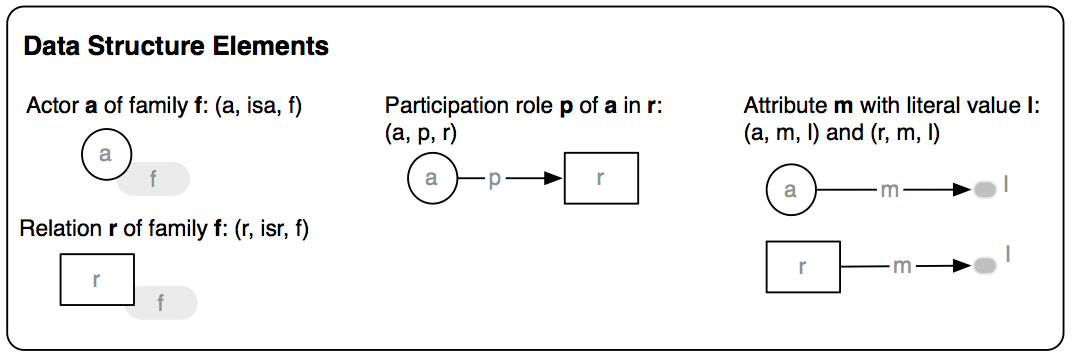
\includegraphics[width=1.0\textwidth]{images/elementos_modelo_mauro.png}
  \caption[Elementos Gráficos SNM]{\emph{Elementos Gráficos SNM}. Desde izquierda a derecha, los 4 bloques de construcción gráfica de una red social: un actor (arriba) y su etiqueta de familia, una relación y su etiqueta de familia, un rol de participación de un actor en una relación y atributos sobre actores y relaciones. Además por cada bloque se muestra la equivalencia en forma de triple.}
  \label{elementos_graficos_snm}
\end{figure}

Dados estos elementos gráficos podemos modelar una red de ejemplo como:

\begin{figure}[H]
  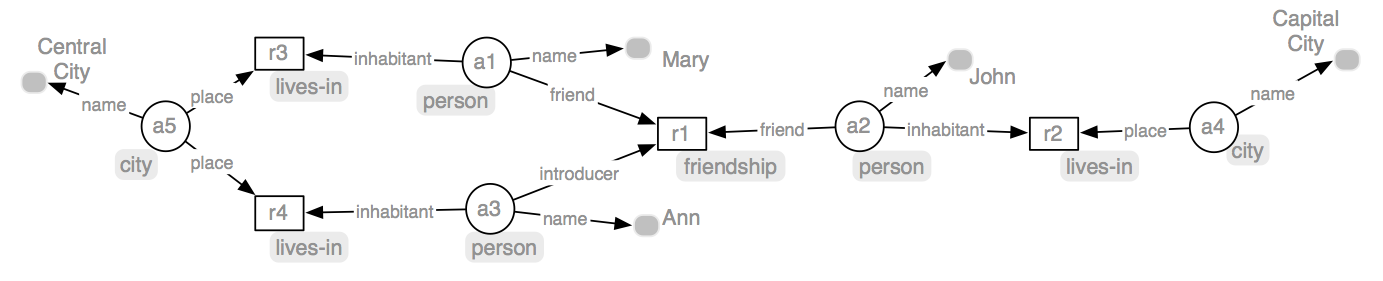
\includegraphics[width=1.0\textwidth]{images/ejemplo_red_social_mauro.png}
  \caption[Ejemplo Red Social de Amistad en SNM]{\emph{Ejemplo Red Social de Amistad en SNM}. Una red social representando relaciones de amistad (nodos cuadrados) entre Mary y John, quienes fueron presentados por Ann (los actores se muestran como nodos circulares y sus atributos como puntos grises). Las ciudades de residencia también son representadas como actores.}
  \label{ejemplo_red_snm}
\end{figure}

% subsection representación_gráfica (end)

\subsection{Representación Como Triples} % (fold)
\label{sub:representacion_como_triples}

El modelo SNM, al ser en una representación de grafo, es posible representarlo como triples y vice-versa (la demostración se encuentra en la memoria de Mauro\cite{tesismauro}). Lo cual es particularmente útil para usar este modelo dentro de un contexto de bases de datos relacionales, razón por la cual veremos una de estas transformaciones a continuación.

Es posible traducir una red social dada, representada como tres conjuntos de triples $(N, R, M)$, en donde $N$ es el conjunto de triples de \emph{Tipos}, $R$ el de \emph{Roles} y $M$ de \emph{Atributos}; en una red social generalizada $G$ con el siguiente algoritmo que produce un nodo o arco por cada triple:

\begin{itemize}
  \item Para cada triple $(\nu_A(a), isa, f_A(A_i))$ en $N$, se añade un nodo actor $a$ en $A_i$.
  \item Para cada triple $(\nu_T(t), isr, f_T(T_i))$ en $N$, se añade un nodo de relación $t$ a $T_i$.
  \item Para cada triple $(\nu_A(u), \epsilon_{AT}(e), \nu_T(v))$ en $R$, se añade un arco de participación $e$ a $E_{AT}$ con nodos finales $u \in A$ y $v \in T$.
  \item Para cada triple $(\nu_A(u), \epsilon_{AC}(e), \nu_C(v))$ en $M$, se añade un nodo de atributo $v$ a $C$, y su arco de significado $e$ a $E_{AC}$ con nodos finales $u \in A$ y $v \in C$.
  \item Para cada triple $(\nu_T(u), \epsilon_{TC}(e), \nu_C(v))$ en $M$, se añade un nodo de atributo $v$ a $C$, y su arco de significado $e$ a $E_{TC}$ con nodos finales $u \in T$ y $v \in C$.
\end{itemize}

Por ejemplo se muestra la siguiente tabla que representa este conjunto de triples, que es similar a lo que se tendría en una base de datos relacional para el caso de la red de amistades de la figura \ref{ejemplo_red_snm}.

\begin{table}[h]
    \begin{tabular}{|c|c|c|l|c|c|c|l|c|c|c|}
    \cline{1-3} \cline{5-7} \cline{9-11}
    \multicolumn{3}{ |c| }{N: Typing}           & ~ & \multicolumn{3}{ c| }{R: Roles} & ~ & \multicolumn{3}{ c | }{M: Attributes}              \\ \cline{1-3} \cline{5-7} \cline{9-11}
    a1 & isa       & 'person'     & ~ & a1 & friend     & r1 & ~ & a1 & name          & 'Mary'         \\
    a2 & isa       & 'person'     & ~ & a2 & friend     & r1 & ~ & a2 & name          & 'John'         \\
    a3 & isa       & 'person'     & ~ & a3 & introducer & r1 & ~ & a3 & name          & 'Ann'          \\
    a4 & isa       & 'city'       & ~ & a2 & inhabitant & r2 & ~ & a4 & name          & 'Capital City' \\
    a5 & isa       & 'city'       & ~ & a4 & place      & r2 & ~ & a5 & name          & 'Central City' \\
    r1 & isr       & 'friendship' & ~ & a1 & inhabitant & r3 & ~ & ~  & ~             & ~              \\
    r2 & isr       & 'lives-in'   & ~ & a5 & place      & r3 & ~ & ~  & ~             & ~              \\
    r3 & isr       & 'lives-in'   & ~ & a3 & inhabitant & r4 & ~ & ~  & ~             & ~              \\
    r4 & isr       & 'lives-in'   & ~ & a5 & place      & r4 & ~ & ~  & ~             & ~              \\ \cline{1-3} \cline{5-7} \cline{9-11}
    \end{tabular}
    \caption {Representación en triples de la red social de la figura \ref{ejemplo_red_snm}}
\end{table}

% subsection representación_como_triples (end)

% section social network model (end) 

% section herramientas_elegidas (end)

\section{Arquitectura de la Aplicación} % (fold)
\label{sec:arquitectura_de_la_aplicacion}

\subsection{Arquitectura de Software} % (fold)
\label{sub:arquitectura_de_software}

La solución considera una aplicación para el manejo de grafos, que consta con un back-end que provee servicios para el almacenamiento y persistencia de las redes sociales junto con un front-end el cual despliega la lógica del editor mismo que los usuarios usan en el día a día.\\

Este esquema permite la creación de diversos sistemas distintos que se alimenten de la data generada por la aplicación como programas completamente independientes. Por otro lado, debido a que el front-end de la aplicación usa un framework  client side como EmberJS, el código de este front-end se obtiene inicialmente desde el back-end, para luego correr en el dispositivo del cliente, donde existirá comunicación entre los componentes de la aplicación, vía peticiones HTTP de tipo JSON para la sincronización y almacenamiento de los datos, mencionando además que estas llamadas son todas de forma autenticada, por lo que el trabajo de diversos usuarios no colisiona entre sí. Para mostrar de mejor manera lo recién descrito, se agrega una figura de la arquitectura general de la aplicación y como sus usuarios interactúan con ella.

\begin{figure}[H]
  \centering
  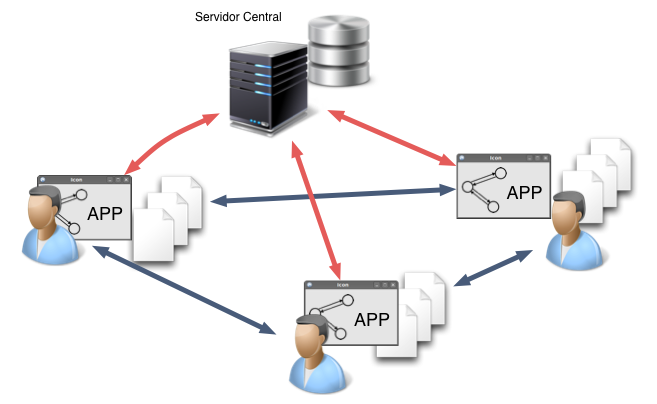
\includegraphics[width=0.8\textwidth]{images/app_distribuida.png}
  \caption[Arquitectura General Aplicación-Usuarios]{\emph{Arquitectura General Aplicación-Usuarios}. en ella se puede observar que la aplicación del lado del cliente se comunica con un servidor central que almacena los datos, pero además diversos usuarios de la aplicación pueden comunicarse independientemente entre ellos por medio de archivos RDF/N3.}
  \label{app_distribuida}
\end{figure}

Los usuarios pueden interactuar entre sí intercambiando información generada entre ellos por medio de los archivos de exportación RDF/N3, esta forma de interacción de los usuarios de la aplicación es una aproximación inicial a este problema en particular, debido a las restricciones de tiempo del trabajo de memoria, junto con la gran cantidad de otros problemas y detalles que solucionar primero.\\

Este esquema general, debido a la calidad de proyecto de código abierto, puede ser replicado por 3eros, en donde puedan instalar su propio servidor de la aplicación de manera de tener un ambiente de redes sociales privados, como puede ser el caso de una universidad en particular.\\

Según lo que se comentó anteriormente, esta arquitectura posee la potencialidad de integrar diversas otras aplicaciones que usen este tipo de datos de redes sociales, sin embargo, como la lectura en sí de los datos sólo se hace en el lado del cliente, en el servidor no se entrega ningún dato que no pertenezca a su propio cliente, de esta forma, no hay conflictos con la privacidad de la información, donde la aplicación entrega la funcionalidad al usuario y este se hace cargo del uso que hace de esta.\\

En una vista más en detalle de la aplicación, para explicar de mejor manera como funciona el software internamente, a continuación se muestra un diagrama de cómo este está estructurado por sus componentes.

\begin{figure}[H]
  \centering
  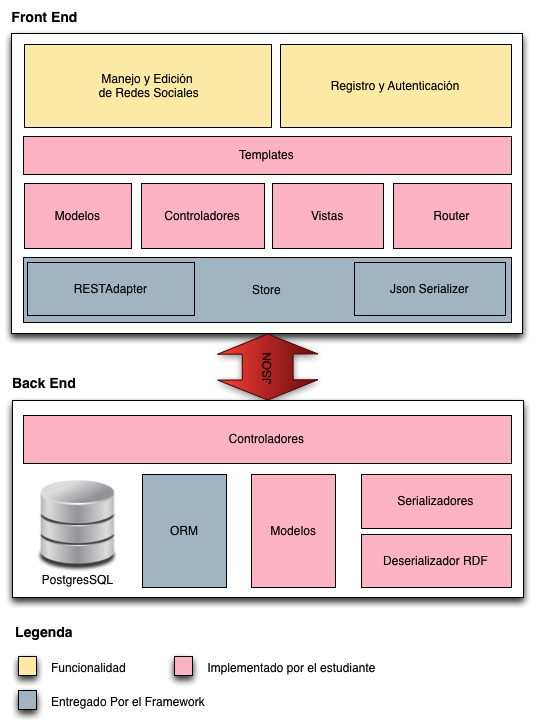
\includegraphics[width=0.7\textwidth]{images/arquitectura_de_software.png}
  \caption[Arquitectura de la Aplicación]{\emph{Arquitectura de la Aplicación}. en una vista de componentes, donde algunos de estos son entregados por las herramientas utilizadas.}
  \label{arquitectura_de_software}
\end{figure}

Desde punto de vista del back-end, se definen los \emph{modelos} correspondientes a la aplicación (Node, Role, etc) los cuales se definen como clases, luego el \textbf{ORM} es el componente encargado de convertir ciertos métodos del modelo en código SQL que se envía a \textbf{PostgreSQL}, de esta forma, al trabajar con los modelos no es necesario escribir nada de SQL, haciendo la programación mucho más fácil. La interfaz que posee el back-end la conforman un conjunto de \emph{controladores}, quienes son los encargados de responder las peticiones HTTP que llegan al servidor, en donde interactúan con los modelos y como se trata de en su mayoría de API JSON, es necesario definir componentes que representan un modelo de la base de datos en formato JSON, esto lo hacen los \emph{serializadores}. Por su parte, hay un \emph{deserializador RDF} que hace el proceso inverso y crea modelos a partir del contenido de un archivo RDF, lo que se usa en la importación de redes sociales.\\

Para el front-end, en donde se definen las interfaces gráficas con las que el usuario trabaja, además de definir la lógica correspondiente a la aplicación misma, esta se abstrae casi completamente del back-end siendo su único punto de conexión las API JSON en donde intercambian mensajes hacia ambos lados, donde en el caso del front-end esto lo maneja un componente de EmberJS llamado \emph{Store}.\\

Se observa en la figura~\ref{arquitectura_de_software} que existen modelos, en el front-end que son los mismos presentes en el back-end, sin embargo difieren ligeramente en la lógica de operaciones con respecto a la edición y alternativamente el back-end puede cambiar completamente y mientras la API se respete, los modelos del front-end no son afectados de ninguna forma.\\

\subsection{Entidades} % (fold)
\label{sub:entidades}

Para comprende de mejor manera la aplicación y los diferentes procesos, es necesario especificar qué entidades existen y qué rol cumplen dentro de la aplicación, estas están con sus nombres en inglés, idioma que se usó para escribir el código de la aplicación.\\

  \begin{itemize}
    \item \textbf{User}: representa a un usuario del sistema, este cuenta con la información necesaria para que un usuario de la aplicación pueda autentificarse dentro del sistema y de esa forma entregarle los permisos necesarios para realizar operaciones sobre sus redes sociales.
    \item \textbf{Social Network}: es la unidad principal dentro de la aplicación, es la entidad que agrupa toda la información que se desea plasmar dentro de la aplicación y representa al grafo completo que forma la red social.
    \item \textbf{Node}: es una unidad atómica dentro de una red social que tiene un \emph{tipo} que puede ser \textbf{Actor} o \textbf{Relación}, dado que ambos son equivalentes dentro del modelo de Mauro~\cite{tesismauro}. Un nodo tiene un atributo por defecto y opcional llamado \emph{name} y además puede estar asociados a familias. En general se refiere a \emph{Actor} o \emph{Relación} cuando se necesita hacer una distinción entre ellos o simplemente \emph{Nodo} cuando se habla de ambos.
    \item \textbf{Family}: una familia representa un conjunto para clasificar en tipos a nodos, las familias por su parte cuentan con un tipo que indica a que tipo de nodo pueden ser asociadas (Actor o Relación), junto a esto tienen algunas opciones de presentación, como el color con que se mostrarán los nodos pertenecientes a una familia.
    \item \textbf{Node Attribute}: son los atributos de un nodo, representados como un par key-value, cuyo nombre no fue \emph{Attribute} para evitar conflictos de nombres con los frameworks de desarrollo.
    \item \textbf{Role}: representa la participación de un \emph{Actor} dentro de una \emph{Relación}. Posee un nombre que es opcional para identificar un rol específico dentro de una relación, por ejemplo: la persona que presenta a otras 2 en una relación de amistad.
  \end{itemize}

% subsection entidades (end)

\subsection{Diseño de la Base de Datos} % (fold)
\label{sub:diseno_de_la_base_de_datos}

A partir de las entidades definidas anteriormente, a continuación se presenta la representación en la base de datos, en este caso PostgresSQL, en donde las relaciones siguen la convención de Ruby on Rails, es decir, \texttt{model\_name\_id}, los nombres de tabla, son iguales al nombre del modelo en plural en minúscula, ej: la tabla del modelo \emph{Node} se llama \emph{nodes}, además Rails crea campos de tiempo de creación y actualización que los maneja internamente como ayuda al desarrollo.

\begin{figure}[H]
  \centering
  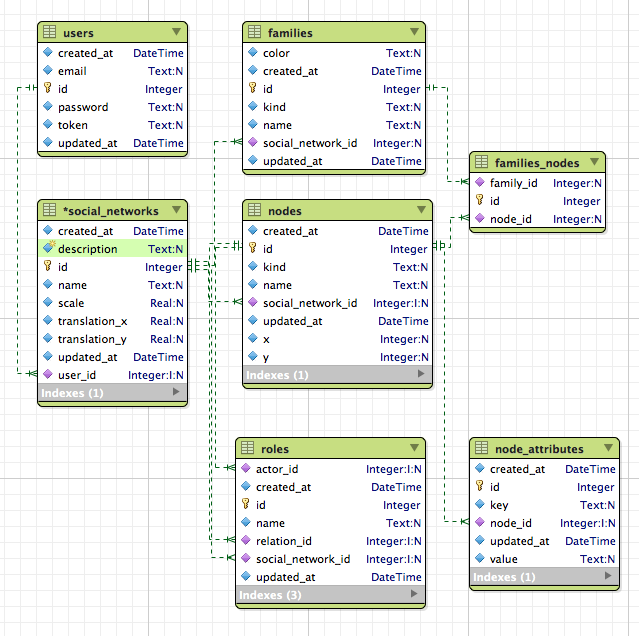
\includegraphics[width=1.0\textwidth]{images/schema_db.png}
  \caption[Esquema Base de Datos de La Aplicación]{\emph{Esquema Base de Datos de La Aplicación}. Una visualización del esquema de la base de datos con sus relaciones correspondientes.}
  \label{schema_db}
\end{figure}

Esta representación se basa en la descrita por el modelo de Mauro en la sección \ref{sub:representacion_como_triples}, con las extensiones correspondientes al dominio de este problema, que se listan a continuación:

  \begin{enumerate}
    \item El modelo de Node, contiene campos de posición x e y para almacenar su posición en el canvas.
    \item El modelo de Social Network, no existente en el modelo de Mauro, se crea con el fin de agrupar la entidad de una red social, donde tiene detalles de la misma, además de algunos campos para recordar preferencias de visualización, como por ejemplo la escala y la translación del canvas.
    \item Las familias poseen un campo de color para visualizar los nodos que pertenecen a ella.
    \item La tabla \emph{families\_nodes} es la forma de Ruby on Rails de crear relaciones de N a M.
    \item La tabla de roles posee también una referencia a su red social, debido a de esta forma se puede obtener de una manera simple, toda la información de una red social en una sola query, sin problemas de duplicidad por las referencias al rol por parte de actores y relaciones.
    \item La tabla \emph{node\_attributes} posee un nombre que evita conflictos de nombre con las herramientas usadas en el desarrollo.
  \end{enumerate}

En relación a los campos visuales dentro de los modelos, es perfectamente viable tener un modelo separado para manejar toda la información que se refiere a estilos, pero debido a que esta es muy poca, se optó por tenerla en sus mismos modelos por simplicidad.

% subsection diseño_de_la_base_de_datos (end)

% section arquitectura_de_la_aplicación (end)
